\documentclass[table]{beamer}
\usetheme{Boadilla}

\usepackage[utf8]{inputenc}
\usepackage[full]{textcomp}
\usepackage[T1]{fontenc}
\usepackage{graphicx}
\usepackage{algorithm,algpseudocode}
\usepackage{color}
\usepackage{tikz,pgf}
\usetikzlibrary{matrix,shapes,arrows,shadows,calc,decorations.markings,fit}
\usepackage{amsmath, amsthm, amssymb}
\usepackage{url}
\usepackage{hyperref}
\usepackage{comment}
\beamertemplatenavigationsymbolsempty

\definecolor{break}{RGB}{197,197,234}

\providecommand{\jlcm}{\mbox{\textit{j}LCM}}
\providecommand{\toppi}{\mbox{\textsc{TopPI}}}
\providecommand{\capa}{\mbox{\textsc{CAPA}} }
\providecommand{\datalyse}{\mbox{\textsc{Datalyse}} }


\title[Soutenance de thèse]{Fouille et classement d'ensembles fermés dans des données transactionnelles de grande échelle}
\author[M. Kirchgessner]{\scriptsize{Thèse préparée au sein de l'équipe SLIDE du LIG\\ pour le titre de Docteur de l'Université de Grenoble, présentée par}\\\vspace{1em}\normalsize{Martin Kirchgessner}}
\institute[LIG]{
  Sous la direction de Sihem Amer-Yahia et Vincent Leroy
}
\date[26 Septembre 2016]{}

\begin{document}

\begin{frame}[plain]
	\titlepage
  \vspace{-2em}
  \begin{columns}[c]
    \column{.35\textwidth}
    \includegraphics[height=1cm,keepaspectratio]{fig/CNRSfilaire-grand.jpg}
    \column{.3\textwidth}
    \includegraphics[height=1.5cm,keepaspectratio]{logo-uga.png}
    \column{.3\textwidth}
    \hfill
    \includegraphics[height=1cm,keepaspectratio]{fig/LIG_coul.pdf}
  \end{columns}
\end{frame}

\begin{frame}[t]{Le projet Datalyse}
  Collaboration avec le Groupe Les Mousquetaires, acteur majeur de la grande distribution en France et en Europe.
  \vspace{1em}
  \begin{columns}[c]
    \column{.7\textwidth}
      Objectif : étudier les habitudes d'achat.
      \\\vspace{1em}
      Méthode : fouille d'associations entre items.
    \column{.3\textwidth}
      \includegraphics[width=0.8\textwidth]{fig/logoIM.jpg}
  \end{columns}
  \vspace{1em}
  Exemples :
  \begin{table}
    \centering
    \def\arraystretch{3}
    \begin{tabular}{rl}
    Algues nori, Wasabi, Sauce Soja  $\rightarrow$ & Riz à Suhis\\
    {\em Nord, $< 35$ ans, Homme}  $\rightarrow$ & {\em Sodas}
  \end{tabular}
  \end{table}
\end{frame}

\begin{frame}{"de grande échelle"}
  Sur l'année 2013:
  \begin{itemize}
    %\tightlist
    \item 290,734,163 tickets
    \item 222,228 produits
    \item 9,267,961 clients
    \item 1884 magasins à travers la France
  \end{itemize}
\end{frame}

\begin{frame}{Distribution en longue traine}
  \begin{center}
    \begin{tikzpicture}
      \node[anchor=south west,inner sep=0] at (0,0) {\includegraphics[width=.5\linewidth]{fig/freq_distrib.pdf}};
      \draw[red,ultra thick,->] (2, 5) -- (1.2, 5);
      \node<1>[align=left,anchor=west](top) at (2,5) {Emmental rapé \\ Sacs plastiques};
      \node<2>[align=left,anchor=west](top) at (2,5) {Radiohead \\ The Beatles};
      \draw[red,ultra thick,->] (4.5, 2) -- (3.5, 1);
      \node<1>[align=left,anchor=west](tail) at (4.5, 2) {Riz à suhis \\ Guacamole \\ \ldots};
      \node<2>[align=left,anchor=west](tail) at (4.5, 2) {Louise Attaque \\ Booka Shade \\ \ldots};
      \node(z) at (0.4, 0.5) {0};
      \node<1>(x) at (0.4, 5.5) {$10^6$};
      \node<2>(x) at (0.4, 5.5) {$10^5$};
      \node(x) at (0.4, 2) {$10^4$};
      \node<1>(y) at (5.5, 0.3) {$10^5$};
      \node<2>(y) at (5.5, 0.3) {$10^6$};
    \end{tikzpicture}
  \end{center}
  \only<1>{
    $\mathit{Support}(\mathit{item}) = $ Nombre de transactions contenant cet item.
  }
  \only<2>{
    \begin{footnotesize}
      {\em Anatomy of the long tail: ordinary people with extraordinary tastes},\\
      Goel, Broder, Gabrilovich, Pang @ WSDM'10
    \end{footnotesize}
  }
\end{frame}

\begin{frame}{Problematiques de la recherche d'associations significatives}
  \begin{itemize}
    \item Couverture
      \begin{itemize}
        \item Etudier les associations concernant {\em n'importe quel} item
      \end{itemize}
    \vspace{1em}
    \item Passage à l'échelle
      \begin{itemize}
        \item Analyser des millions de transactions
      \end{itemize}
    \vspace{1em}
    \item Qualité
      \begin{itemize}
        \item Indiquer les associations remarquables
      \end{itemize}
  \end{itemize}
\end{frame}


\begin{frame}{Contributions}
  \begin{itemize}
    \item Couverture et passage à l'échelle
      \begin{itemize}
        \item Fouille item-centrée avec \toppi
      \end{itemize}
    \vspace{1em}
    \item Qualité
      \begin{itemize}
        \item Comparaison des mesures de qualité avec \capa
      \end{itemize}
  \end{itemize}
\end{frame}






\section{Fouille item-centrée avec \toppi}

{
\setbeamercolor{background canvas}{bg=break}
\begin{frame}{}
  Fouille item-centrée avec \toppi
\end{frame}
}

\begin{frame}[t]{Itemsets fréquents et longue traine}
  \begin{center}
    \only<1>{ \includegraphics[width=.7\linewidth]{fig/freq_distrib_standard.pdf} }
    \only<2>{ \includegraphics[width=.7\linewidth]{fig/freq_distrib_standard_low.pdf} }
  \only<3>{
    \begin{tabular}{|c|l|}
      \hline
      {\bf Support(P)} & {\bf P} \\\hline
      861 304 &	Emmental rapé, Crème fraîche 30\% \\
      793 310 &	Emmental rapé, 10 Oeufs \\
      747 539 &	Sucre en poudre, Farine \\
      652 493 &	Emmental rapé, Beurre \\
      616 696 &	Sucre en morceaux, Sucre en poudre \\
      597 144 &	Emmental rapé, Lardons fumés \\
      549 742 &	Emmental rapé, Jambon \\
      542 979 &	Emmental rapé, Sucre en morceaux \\
      508 593 &	Emmental rapé, Soda 1.5L \\
      481 942 &	Emmental rapé, Huile de tournesol \\
      \multicolumn{2}{|c|}{\ldots}
    \end{tabular}
  }
  \end{center}
\end{frame}

\begin{frame}{Fouille item-centrée avec \toppi}
  \begin{enumerate}
    \item Fouille item-centrée ?
    \item Etat de l'art
    \item L'algorithme
    \item Expériences
    \item Distribuer \toppi{} sur MapReduce
  \end{enumerate}
  \vfill
  \begin{footnotesize}
    {\em TopPI: An Efficient Algorithm for Item-Centric Mining.}\\
    Kirchgessner, Leroy, Termier, Amer-Yahia, Rousset @ DaWaK'16 p.19-33 \\
    \vspace{1em}
    {\em TopPI: An Efficient Algorithm for Item-Centric Mining.}\\
    Leroy, Kirchgessner, Termier, Amer-Yahia --- à paraître dans {\em Information Systems}.
  \end{footnotesize}
\end{frame}


\begin{frame}[t]{Fouille item-centrée}
  \begin{center}
    \begin{tikzpicture}
      \node[inner sep=0] at (0,0) {\includegraphics[width=.35\linewidth]{fig/freq_distrib_standard-simple.pdf}};
      \node[inner sep=0] at (6,0) {\includegraphics[width=.35\linewidth]{fig/freq_distrib_toppi.pdf}};
      \draw[red,ultra thick,->] (2.5, 0) -- (3.5, 0);
    \end{tikzpicture}
  \end{center}
\end{frame}
% TODO : penser à dire "définir les ensembles à calculer ainsi rend la couverture complète faisable"
% au lieu de produire des milliards d'itemsets pour rien,
% j'en produit que k * |I| et idéalement je parcoure que ceux là



\begin{frame}[t]{Une nouvelle sémantique pour la fouille d'itemsets}
  \begin{footnotesize}
    $t_1$ : {\em Camembert, Saucisses, Compté, Chèvre long, Salade mélangée, Sucre en morceaux} \\
    $t_2$ : {\em Brandade de morue, Boite 6 oeufs, Désodorisant, Lessive, Emmental rapé} \\
    $t_3$ : {\em Haricot vert, Boxer, Nettoyant à moquette, Mouchoirs, Salade mélangée} \\
    \ldots\\
  \pause
  Résultats :
    \begin{columns}[c]
      \setlength{\tabcolsep}{1pt}
      \column{0.5\textwidth}
      \begin{tabular}{|c|l|}
        \multicolumn{2}{c}{$\mathit{top}(\text{Emmental rapé})$} \\ \hline
        Support & Itemset \\ \hline
        9 395 643 & Emmental rapé\\
        861 304 &	Emmental rapé, Crème fraîche\\
        793 310 &	Emmental rapé, 10 Oeufs \\
        652 493 &	Emmental rapé, Beurre \\
        597 144 &	Emmental rapé, Lardons fumés \\
        \hline
      \end{tabular}

      \column{0.5\textwidth}
      \begin{tabular}{|c|l|}
        \multicolumn{2}{c}{$\mathit{top}(\text{Crème choc.})$} \\ \hline
        Support & Itemset \\ \hline
        $581 042$ & Crème choc. \\
        $58 569$ & Crème choc., Crème à la vanille \\
        $32 701$ & Crème choc., Emmental rapé 200g \\
        $30 451$ & Crème choc., Cola 1.5L\\
        $29 671$ & Crème choc., Beurre doux\\
        \hline
      \end{tabular}
    \end{columns}
    \begin{center}
    \begin{tabular}{|c|l|}
      \multicolumn{2}{c}{$\mathit{top}(\text{Riz à sushis})$} \\ \hline
      Support & Itemset \\ \hline
      14887  & Riz à sushis \\
      5935   & Riz à sushis, Algues nori \\
      3669  & Riz à sushis, Vinaigre de riz \\
      1843   & Riz à sushis, Algues nori, Vinaigre de riz \\
      1762   & Riz à sushis, Wasabi \\
      \hline
    \end{tabular}

% TODO placer correct
    \ldots

    \end{center}


  \end{footnotesize}
\end{frame}

\begin{frame}{Méthodes existantes}
  \pause
  \begin{block}{Par post-processing}
    \begin{enumerate}
      \item Fouiller tous les itemsets fréquents ($minsup = 2$),
      \item Insérer chaque itemset dans les $top(i)$ concernés.
    \end{enumerate}
  \end{block}
  \pause
  \begin{block}{Par pre-processing (méthode de référence)}
    Pour chaque item $i$:
    \begin{enumerate}
      \item Instanciation de ${\cal D}[i]=\{t \in {\cal D} | i \in t\}$
      \item Exécution de TFP sur ${\cal D}[i]$, qui produit directement $\mathit{top}(i).$
    \end{enumerate}
  \end{block}
  \vfill
  \begin{footnotesize}
    {\em Mining top-k frequent closed patterns without minimum support.}\\
    Han, Wang, Lu, Tzvetkov @ ICDM'02
  \end{footnotesize}
\end{frame}


\begin{frame}[t]{Notre approche : \toppi}
  \begin{enumerate}
    \item<1-> Obtenir tous les $\mathit{top}(i)$ en une exécution
    \item<2-> Un parcours intelligent du treillis des itemsets
    \item<3-> Limite la fouille aux itemsets potentiellement dans un $\mathit{top}(i)$
    \item<4-> Répartition des branches entre les threads
  \end{enumerate}
  \only<1>{
    \begin{center}
      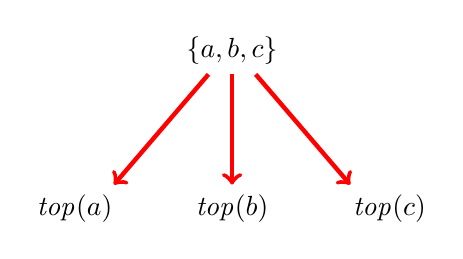
\begin{tikzpicture}
        \node(abc) at (0, 0) {$\{a,b,c\}$};
        \node(a) at (-2, -2) {$\mathit{top}(a)$};
        \node(b) at (0, -2) {$\mathit{top}(b)$};
        \node(c) at (2, -2) {$\mathit{top}(c)$};
        \draw[red,ultra thick,->] (-0.3, -0.3) -- (-1.5, -1.7);
        \draw[red,ultra thick,->] (0, -0.3) -- (0, -1.7);
        \draw[red,ultra thick,->] (0.3, -0.3) -- (1.5, -1.7);
      \end{tikzpicture}
    \end{center}
  }
  \only<2->{
  {
  \begin{center}
  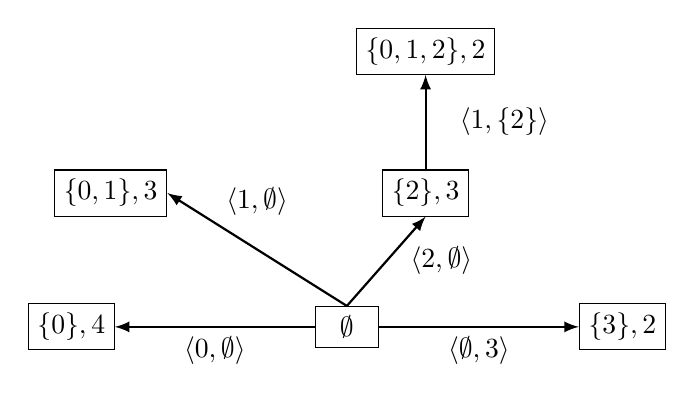
\begin{tikzpicture}[>=latex]
		\node (empty) [draw,rectangle,minimum width = .8cm,minimum height=.5cm] at (0,0) {$\emptyset$};
		\node (0)     [draw,rectangle,minimum width = .8cm,minimum height=.5cm] at (-3.5,0) {$\{0\},4$};
		\node (1)     [draw,rectangle,minimum width = .8cm,minimum height=.5cm] at (-3,1.7) {$\{0,1\},3$};
		\node (2)     [draw,rectangle,minimum width = .8cm,minimum height=.5cm] at (1,1.7) {$\{2\},3$};
		\node (012)   [draw,rectangle,minimum width = .8cm,minimum height=.5cm] at (1,3.5) {$\{0,1,2\},2	$};
		\node (3)     [draw,rectangle,minimum width = .8cm,minimum height=.5cm] at (3.5,0) {$\{3\},2$};
		\draw [->,thick] (empty.west) -- (0.east) node[below, midway] {$\langle 0, \emptyset\rangle$};
		\draw [->,thick] (empty.north) --(1.east) node[above, midway, yshift=0.3cm] {$\langle 1, \emptyset\rangle$};
		\draw [->,thick] (empty.north)--(2.south) node[above, midway, xshift=0.7cm, yshift=-0.3cm] {$\langle 2, \emptyset\rangle$};
		\draw [->,thick] (empty.east)--(3.west) node[below, midway] {$\langle\emptyset, 3\rangle$};
		\draw [->,thick] (2.north)--(012.south) node[above, midway, xshift=1cm, yshift=-0.3cm] {$\langle 1, \{2\}\rangle$};
	\end{tikzpicture}
  \end{center}
  }
  }
  \only<2>{
  \vfill
  \begin{footnotesize}
    {\em LCM ver. 2: Efficient mining algorithms for frequent/closed/maximal itemsets.}\\
    Uno, Kiyomi, Arimura @ FIMI'04
  \end{footnotesize}
  }
  \only<4>{
  \vfill
  \begin{footnotesize}
    {\em Discovering closed frequent itemsets on multicore.}\\
    Négrevergne, Termier, Méhaut, Uno @ HPCS'10
  \end{footnotesize}
  }
\end{frame}


\begin{frame}{\toppi, un algorithme rapide}
  \begin{block}{Temps d'exécution ($k=50$)}
    \centering
    \begin{tabular}{|l|c|c|c|c|}
      \hline
      {\bf Données}    & $|{\cal I}|$ & $|{\cal D}|$ & {\bf Taille} & {\bf Temps} \\\hline
      \textit{Tickets} & $222,228$ & $290,734,163$ & 24GB          & 4 min. \\\hline
      \textit{Tickets, par client} & $222,228$ & $9,267,961$ & 13.3GB           & 11 min. \\\hline
      \textit{LastFM}  & $1,206,195$ & $1,218,831$ & 277MB          & 2 min. \\\hline
      \textit{WebDocs} & $5,267,656$ & $1,692,082$ & 1.4GB           & 8 heures \\\hline
    \end{tabular}
  \end{block}

  Environnement expérimental :
  \begin{itemize}
    \item 32 threads en parallèle
    \item 128 GB de RAM
  \end{itemize}
\end{frame}
% TODO: insister sur le fait que dans WebDocs les itemsets sont plus longs


\begin{frame}{\toppi, distribué sur cluster MapReduce}
  Plus de CPUs pour l'énumération d'itemsets.
  \\\vspace{1em}
  \pause
  \begin{block}{Pas de calculs redondants}
    \begin{itemize}
      \item L'ensemble des items $\cal I$ est partitionné en {\em groupes} : un par machine.
      \item Chaque machine produit une partition des résultats
    \end{itemize}
    \end{block}
    \pause
    \begin{block}{Pas de calculs inutiles}
      \begin{itemize}
        \item Complétion des $\mathit{top}(i)$ en deux étapes
        \item Conserve l'efficacité de l'élagage
      \end{itemize}
  \end{block}
\end{frame}

\begin{frame}{{\toppi} sur cluster MapReduce}
  Sur le cluster ``edel'' de Grid5000.\\\vspace{1em}
  WebDocs, $k=10$ :
  \begin{itemize}
    \item 4570s avec 32 machines (8 threads chacune)
    \item 2641s avec 64
  \end{itemize}
\end{frame}

\begin{frame}{{\toppi} sur cluster MapReduce}
  \begin{figure}
  	\centering
  	\includegraphics[width=0.8\textwidth]{../fig/toppi/hadoop-speedup/supermarket-s2-k1000-t8.pdf}
  \end{figure}
  \textit{Supermarket}, $k=1000$.
\end{frame}

\begin{frame}{{\toppi} sur cluster MapReduce}
  \begin{figure}
  	\centering
  	\includegraphics[width=0.8\textwidth]{../fig/toppi/hadoop-speedup/supermarket-s2-k1000-t8-cumulatedMiningTime.pdf}
  \end{figure}
  \textit{Supermarket}, $k=1000$, temps CPU cumulé passé à la fouille
\end{frame}




\begin{frame}{\toppi}
  \begin{itemize}
    \item Une sémantique adaptée aux longues traines
      \begin{itemize}
        \item Un (unique) paramètre, $k$
        \item Résultats complets et organisés intuitivement (par item)
        \item Applicable dans différents domaines (Web, grande distribution, \ldots)
      \end{itemize}
    \vspace{1em}
    \item Un algorithme qui passe à l'échelle
    \begin{itemize}
      \item Sur serveur multi-coeurs
      \item Sur cluster MapReduce
      \item Elaguage très efficace de l'espace des solutions
    \end{itemize}
    \vspace{1em}
    \item Utilisation industrielle
      \begin{itemize}
        \item \url{https://github.com/slide-lig/TopPI}
      \end{itemize}
  \end{itemize}
\end{frame}


















\section{Comparaison de fonctions de tri avec \capa}
{
\setbeamercolor{background canvas}{bg=break}
\begin{frame}{}
  \capa : Comparative Analysis of PAtterns
  % Comment choisir seulement 10 associations à présenter ?
\end{frame}
}


% TODO: est-ce qu'on a pas un produit plus cool ?
\begin{frame}{Le bruit du tri par fréquence}
  Sur 290 millions de tickets :
  \begin{table}
    \begin{tabular}{|c|c|l|}
      \hline
      $k$ & $\mathit{support}(P)$ & $P$  \\\hline
      $1$  & $581042$ & Crème au chocolat \\
      $2$  & $58569$ & Crème au chocolat, Crème à la vanille \\
      $3$  & $32701$ & Crème au chocolat, Emmental rapé 200g \\
      $4$  & $30451$ & Crème au chocolat, Cola 1.5L\\
      $5$  & $29671$ & Crème au chocolat, Beurre doux\\
      $6$  & $29376$ & Crème au chocolat, Emmental rapé 3x70g\\
      $7$  & $24869$ & Crème au chocolat, Emmental rapé 200g Marque B\\
      $8$  & $23032$ & Crème au chocolat, Lait 1/2 écrémé\\
      $9$  & $19929$ & Crème au chocolat, Lait 6x1L\\
      $10$ & $16547$ & Crème au chocolat, Pâte feuilletée\\
      \hline
    \end{tabular}
  \end{table}
\end{frame}

\begin{frame}{Trier des règles d'association}
  39 mesures de qualité dans la littérature.

  \begin{itemize}
    \item Sont-elles vraiment différentes ?
    \item Laquelle choisir ? Pour la grande distribution ?
    \item Comment simplifier l'évaluation par des experts ?
  \end{itemize}
  \vspace{1em}
  %Le service marketing d'Intermarché est prêt à évaluer des mesures de qualité... \\
  %\hfill ... mais pas 39 !

  \vfill
  \begin{footnotesize}
    \setlength{\baselineskip}{-0.5em}
    {\em Interestingness Measures for Data Mining: A Survey.}\\
    Geng, Hamilton, {\em ACM Computer Surveys}, 2006\\
    \medskip
    {\em Association Rule Interestingness Measures: Experimental and Theoretical Studies.}\\
    Lenca, Vaillant, Meyer, Lallich, {\em Quality Measures in Data Mining}, 2007\\
    \medskip
    {\em Beyond Support and Confidence: Exploring Interestingness Measures for Rule-Based\\ Specification Mining.}
    Le, Lo @ SANER'15\\
  \end{footnotesize}
\end{frame}

\begin{frame}{La méthode \capa}
  \begin{block}{Comparative Analysis of PAtterns}
    \begin{enumerate}
      \item Comparaison automatique des mesures\\
      $\rightarrow$ distingue des familles de mesures donnant des classements similaires.
      \item Validation empirique, où les chargées d'étude marketing comparent les familles de classements.
    \end{enumerate}
  \end{block}
  \vfill
  \begin{footnotesize}
    {\em Testing Interestingness Measures in Practice: A Large-Scale Analysis of Buying Patterns.}\\
    Kirchgessner, Leroy, Amer-Yahia, Mishra @ DSAA'16
  \end{footnotesize}
\end{frame}


\begin{frame}[t]{Comparaison automatique des mesures}
  \begin{enumerate}
    \item<1-> Définition de cibles d'étude
    \item<2-> Fouille des associations correspondantes
    \item<3-> Classement d'après les 39 mesures
    \item<4-> Comparaison des classements avec 4 distances
      \only<4>{
      \begin{itemize}
        \item Coefficient de Spearman
        \item $\tau$ de Kendall
        \item Overlap@20
        \item NDCC : {\em Normalized Discounted Correlation Coefficient}
      \end{itemize}
      }
    \item<6-> Regroupement hiérarchique
  \end{enumerate}
  \only<1>{
    \begin{center}
      \item Contraintes sur les ensembles $A \rightarrow B$
    \end{center}
  }

  \begin{scriptsize}
  \only<2>{
    \begin{table}
      \setlength{\tabcolsep}{1pt}
      \centering
      \begin{tabular}{|rl|c|c|}
      \hline
      $A$                   &  $\rightarrow B$   & $\mathit{support}(A)$    & $\mathit{support}(A \cup B)$     \\\hline
      $\{35-49\}$    & $\rightarrow$ {\em Patisserie indus.}   & 66 811 806                &   22 270 602 \\
      $\{35-49\}$    & $\rightarrow$ {\em Boissons}   & 66 811 806                &   16 513 795 \\
      $\{35-49, F\}$ & $\rightarrow$ {\em Patisserie indus.}   & 45 267 831                &   15 089 277 \\
      $\{ F \}$ & $\rightarrow$ {\em Epicerie sucrée }   & 205 330 640                &   112 931 852 \\
      $\{ >64, F$, Rhône-Alpes $\}$ & $\rightarrow$ {\em Crèmerie}   & 6 649 289     &      4 255 545 \\
      \multicolumn{4}{|c|}{\ldots} \\
      \end{tabular}
    \end{table}
  }

  \only<3>{
    \begin{columns}[c]
      \hfill
      \setlength{\tabcolsep}{1pt}
    	\column{.4\textwidth}
          \begin{tabular}{|rl|}
          \hline
          \multicolumn{2}{|c|}{\textbf{Confiance}}               \\\hline
          $\{> 65, F, $ Aube$\}$&$\rightarrow$ {\em Dairy}       \\
          $\{> 65, F, $ Aveyron$\}$&$\rightarrow$ {\em Dairy}       \\
          $\{> 65, F, $ Val de Marne$\}$& $ \rightarrow$ {\em Dairy}       \\
          $\{> 65, F, $ Seine S$^{t}$ Denis$\}$& $ \rightarrow$ {\em Dairy}       \\
          $\{> 65, F, $ Haute Saone$\}$& $ \rightarrow$ {\em Dairy}       \\
          $\{> 65, F, $ Meuse$\}$& $ \rightarrow$ {\em Dairy}       \\
          $\{> 65, *, $ Aube$\}$& $ \rightarrow$ {\em Dairy}       \\
          $\{> 65, F, $ Haute Vienne$\}$& $ \rightarrow$ {\em Dairy}       \\
          $\{> 65, F, $ Maine et Loire$\}$& $ \rightarrow$ {\em Dairy}       \\
          $\{> 65, *, $ Val de Marne$\}$& $ \rightarrow$ {\em Dairy}           \\\hline
          \end{tabular}
    		\column{.4\textwidth}
          \begin{tabular}{|rl|}
          \hline
          \multicolumn{2}{|c|}{\textbf{Piatetsky-Shapiro}}       \\\hline
            $\{*, *, $ Nord$\}$&$\rightarrow$ {\em Liquids}       \\
            $\{*, *, $ Nord$\}$&$\rightarrow$ {\em Soft drinks}       \\
            $\{*, *, $ Nord$\}$&$\rightarrow$ {\em Beers}       \\
            $\{*, *, $ Nord$\}$&$\rightarrow$ {\em Spreads}       \\
            $\{*, F, $ Nord$\}$&$\rightarrow$ {\em Soft drinks}       \\
            $\{*, *, $ Nord$\}$&$\rightarrow$ {\em Imported beers}       \\
            $\{*, F, $ Nord$\}$&$\rightarrow$ {\em Liquids}       \\
            $\{*, F, $ Nord$\}$&$\rightarrow$ {\em Beers}       \\
            $\{*, *, $ Finistere$\}$&$\rightarrow$ {\em Butters}       \\
            $\{*, F, $ Garonne$\}$&$\rightarrow$ {\em Drugstore}          \\\hline
          \end{tabular}
    		\column{.1\textwidth}
        \begin{tabular}{|rl|}
        \hline
        \multicolumn{2}{|c|}{\textbf{$\chi^2$}}      \\\hline
        $\{*, *, $ Somme$\}$&$\rightarrow$ {\em Cut cheese}       \\
         $\{*, F, $ Somme$\}$&$\rightarrow$ {\em Cut cheese}       \\
        $\{> 65, *,$ Morbihan$\}$&$\rightarrow$ {\em Fresh milk}       \\
        $\{> 65, *,$ Somme$\}$&$\rightarrow$ {\em Cut cheese}       \\
        $\{*, *,$ Finistere$\}$&$\rightarrow$ {\em Canned pork}       \\
        $\{*, *,$ Cotes\ d'Armor$\}$&$\rightarrow$ {\em Canned pork}       \\
        $\{> 65, F,$ Morbihan$\}$&$\rightarrow$ {\em Fresh milk}       \\
        $\{*, *,$ Nord$\}$&$\rightarrow$ {\em Beer}       \\
        $\{*, *,$ Nord$\}$&$\rightarrow$ {\em Sparkling liquors}       \\
        $\{*, *,$ Vienne$\}$&$\rightarrow$ {\em Breakfast biscuits}   \\\hline
        \end{tabular}
    \end{columns}
  }
  \end{scriptsize}

  \only<4>{
    \begin{block}{NDCC}
      \begin{itemize}
        \item Calcul inspiré de NDCG
        \item Favorise les classements similaires en tête
      \end{itemize}
    \end{block}
  }

  \only<5>{
    \begin{columns}[t]
      \column{0.25\textwidth}
        \centering
        \includegraphics[width=\linewidth]{fig/similarityMatrix/similarity-Spearman.pdf}
        \\\vspace{1em}
        Coefficient de Spearman
      \column{0.25\textwidth}
        \centering
        \includegraphics[width=\linewidth]{fig/similarityMatrix/similarity-Kendal.pdf}
        \\\vspace{1em}
        $\tau$ de Kendall
      \column{0.25\textwidth}
        \centering
        \includegraphics[width=\linewidth]{fig/similarityMatrix/similarity-O20.pdf}
        \\\vspace{1em}
        Overlap@20
      \column{0.25\textwidth}
        \centering
        \includegraphics[width=\linewidth]{fig/similarityMatrix/similarity-NDCG.pdf}
        \\\vspace{1em}
        NDCC
    \end{columns}
  }

  \only<6>{
    \begin{columns}[t]
      \column{0.25\textwidth}
        \centering
        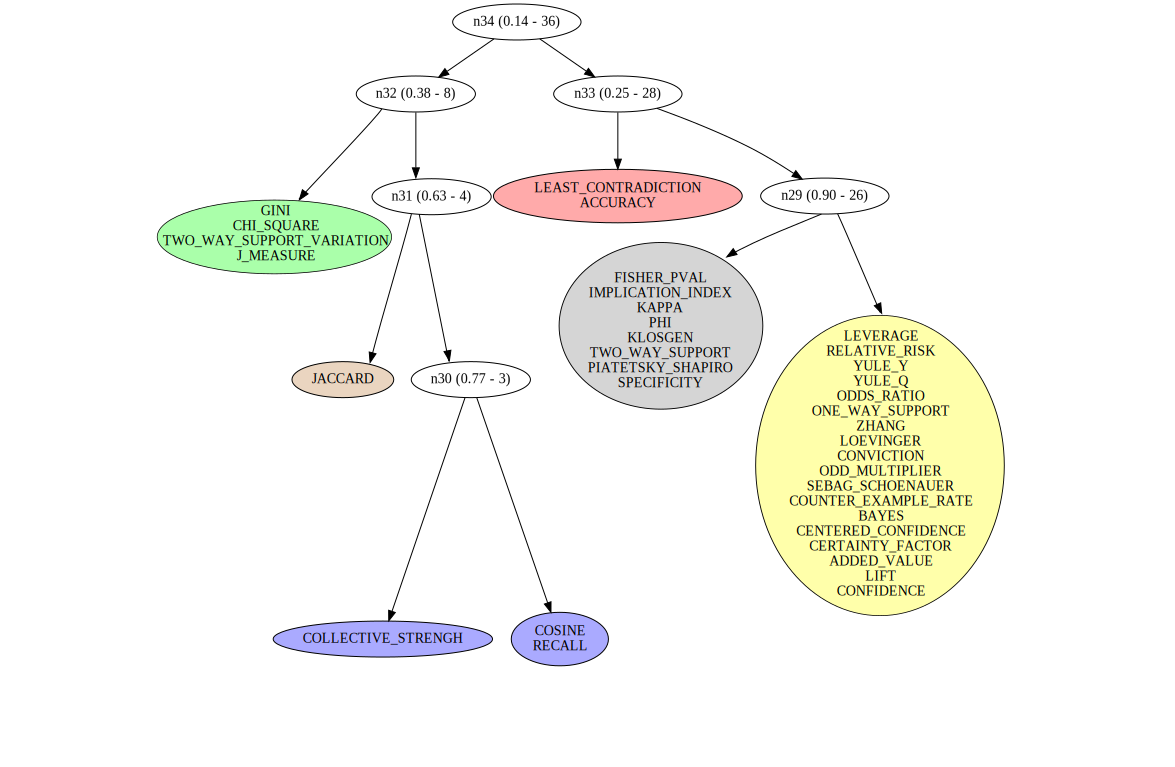
\includegraphics[width=\linewidth]{fig/dendograms/patterns_demo-perTarget-SPEARMAN.pdf}
        \\\vspace{1em}
        Coefficient de Spearman
      \column{0.25\textwidth}
        \centering
        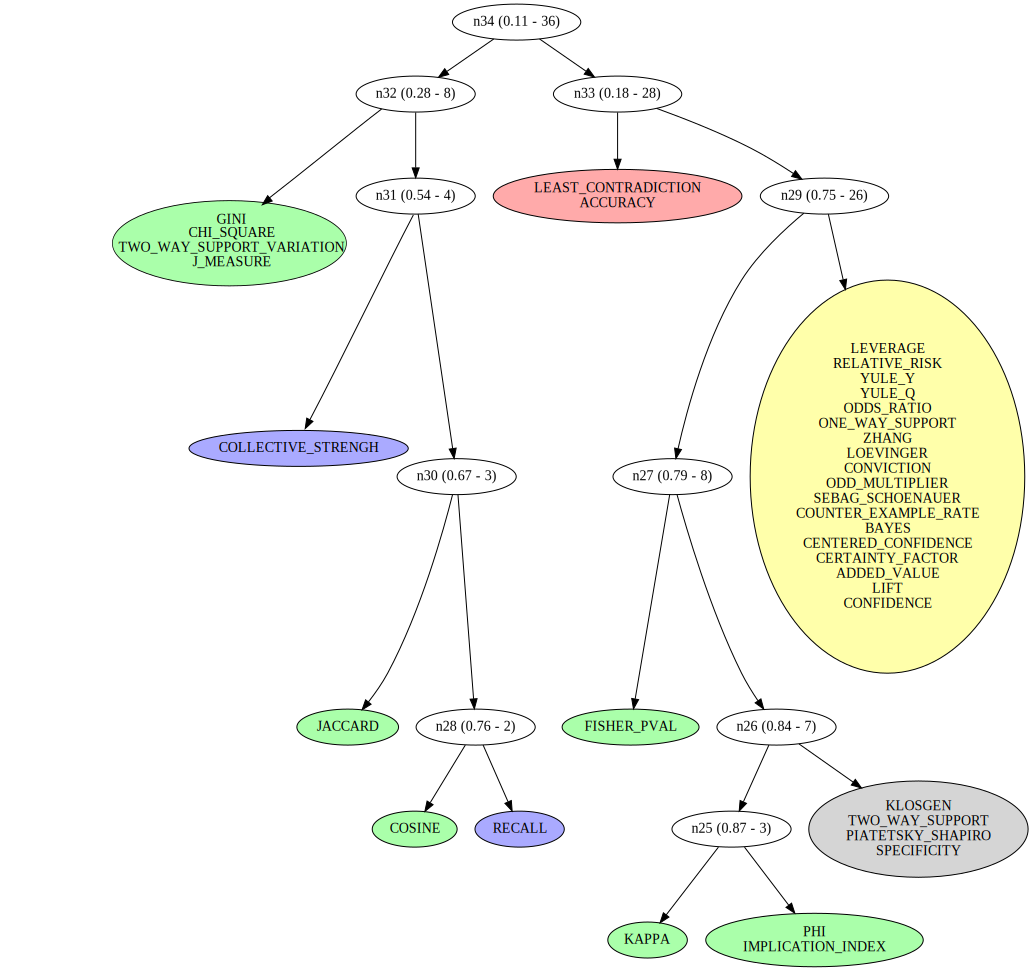
\includegraphics[width=\linewidth]{fig/dendograms/patterns_demo-perTarget-KENDAL.pdf}
        \\\vspace{1em}
        $\tau$ de Kendall
      \column{0.25\textwidth}
        \centering
        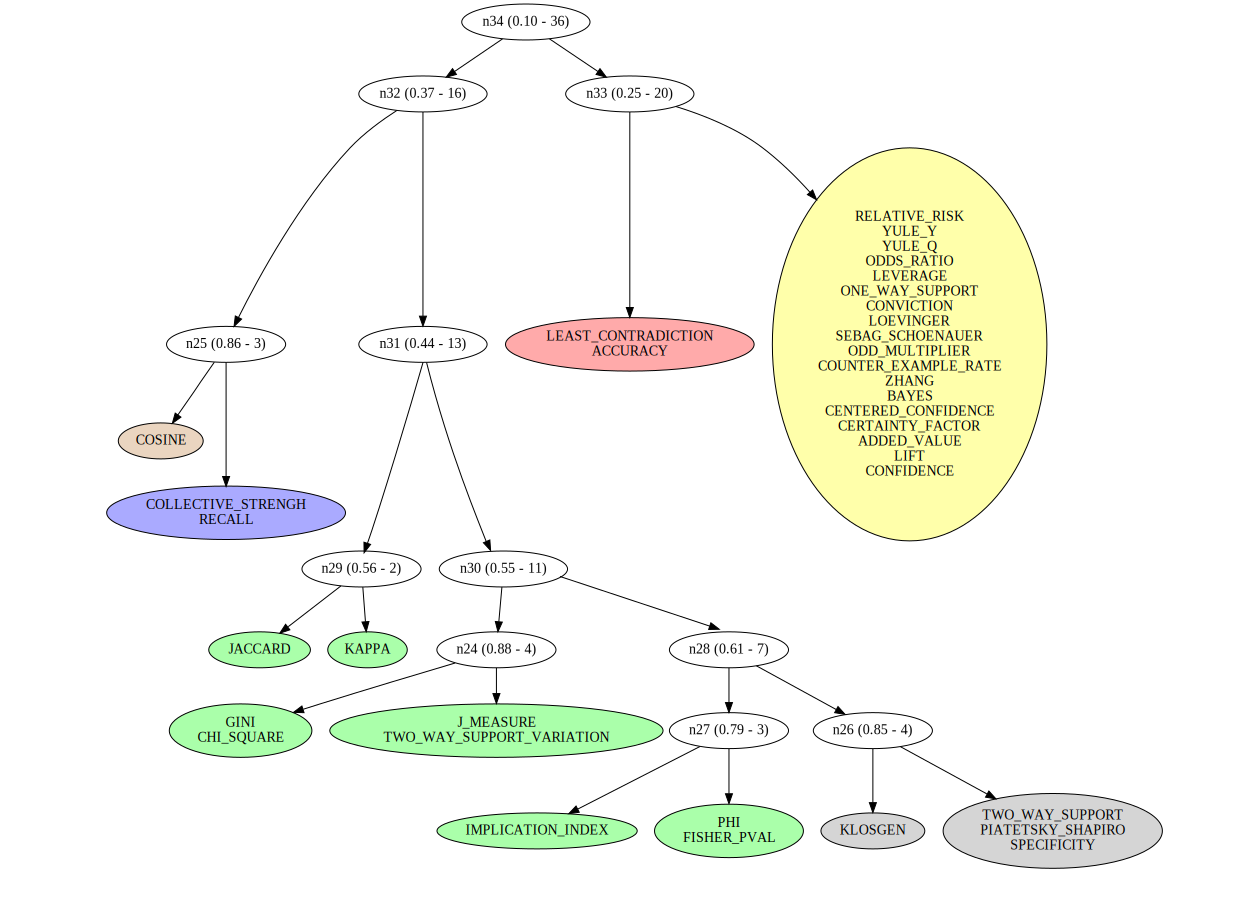
\includegraphics[width=\linewidth]{fig/dendograms/patterns_demo-perTarget-OVERLAP_AT_20.pdf}
        \\\vspace{1em}
        Overlap@20
      \column{0.25\textwidth}
        \centering
        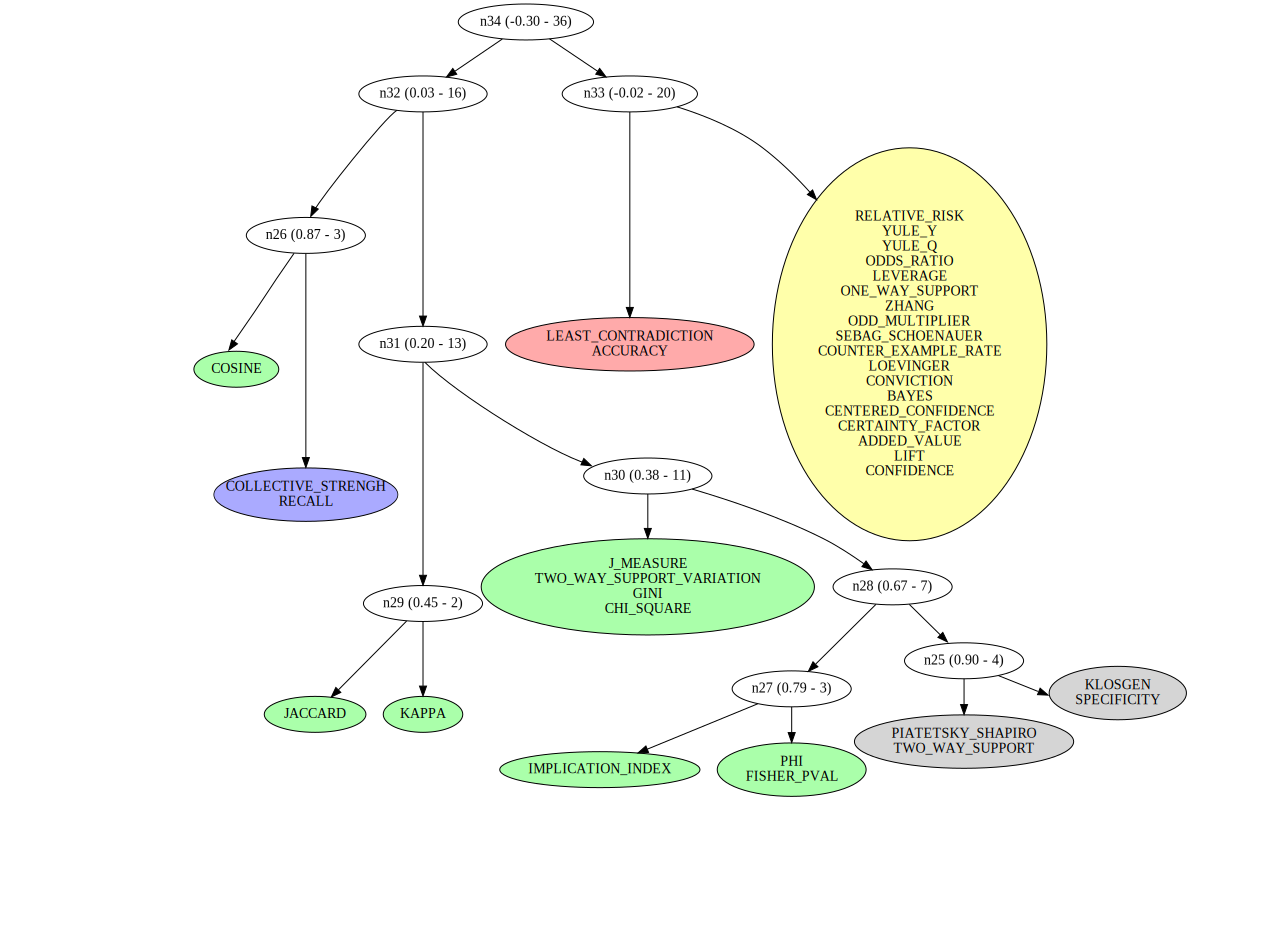
\includegraphics[width=\linewidth]{fig/dendograms/patterns_demo-perTarget-NDCG.pdf}
        \\\vspace{1em}
        NDCC
    \end{columns}
  }
\end{frame}

\begin{frame}[t]{Résultat de la comparaison automatique : 5 familles}
  \centering
  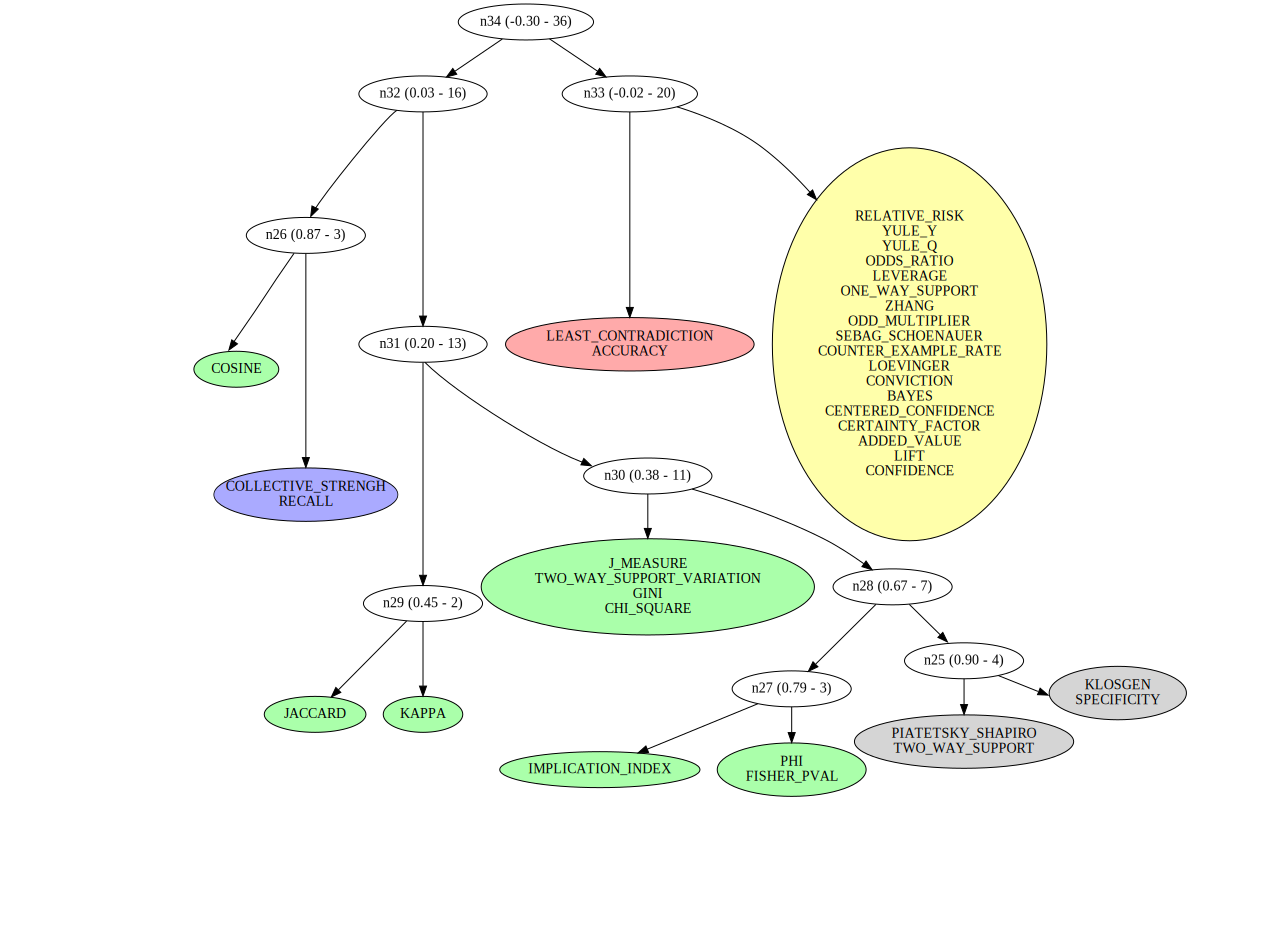
\includegraphics[width=0.8\linewidth]{fig/dendograms/patterns_demo-perTarget-NDCG.pdf}
\end{frame}

\begin{frame}[t]{Etude empirique}
  \begin{figure}
    \centering
    \includegraphics[width=0.7\linewidth]{../fig/screenshot_exploration.png}
  \end{figure}
\end{frame}

\begin{frame}{Etude empirique}
  Capacité d'attention
  \begin{itemize}
    \item 10 à 20 premiers résultats
    \item les derniers, aussi !
  \end{itemize}
  \pause
  Préfèrences :
  \begin{itemize}
    \item Généralement, $G_1$ et $G_2$ (mesures favorisant la confiance)
    \item Pour une cible donnée, $G_3$ et $G_4$
  \end{itemize}
  \vspace{1em}
  L'important est de différencier\\
    \textit{\{crème vanille, emmental rapé\}$\rightarrow$ crème au chocolat} (conf. 32\%)\\
  et\\
    \textit{\{crème vanille\}$\rightarrow$ crème au chocolat} (conf. 31\%)
\end{frame}

\begin{frame}{\capa : généralisation}
  \begin{itemize}
    \item 39 mesures de qualité, mais des classements similaires
    \vspace{1em}
    \item Première étude du genre pour la grande distribution
    \begin{itemize}
      \item Le classement par confiance reste plebiscité
      \item La mesure de Piatetsky-Shapiro retire bien le bruit des ``stars''
    \end{itemize}
    \vspace{1em}
    \item Méthode applicable à d'autres domaines
  \end{itemize}
\end{frame}







\section{Conclusion et perspectives}

{
\setbeamercolor{background canvas}{bg=break}
\begin{frame}{}
  Conclusion
\end{frame}
}


\begin{frame}{Conclusion}
  \toppi
  \begin{itemize}
    \item Un paramètre et des résultats intuitifs
    \item Analyse 300 millions de tickets en quelques minutes
      \begin{itemize}
        \item 47000 par Agrawal \& Srikant en  1994 avec APriori
      \end{itemize}
    \item Speedup linéaire, version distribuée
  \end{itemize}
  \vspace{0.5em}
  \capa
  \begin{itemize}
    \item Bonne présentation des résultats
    \item Permet de choisir un post-traitement
  \end{itemize}
  \vfill
  \begin{footnotesize}
    \setlength{\baselineskip}{-0.5em}
    {\em TopPI: An Efficient Algorithm for Item-Centric Mining.}\\
    Kirchgessner, Leroy, Termier, Amer-Yahia, Rousset @ DaWaK'16 p.19-33 \\
    \medskip
    {\em TopPI: An Efficient Algorithm for Item-Centric Mining.}\\
    Leroy, Kirchgessner, Termier, Amer-Yahia --- à paraître dans {\em Information Systems}.\\
    \medskip
    {\em Testing Interestingness Measures in Practice: A Large-Scale Analysis of Buying Patterns.}\\
    Kirchgessner, Leroy, Amer-Yahia, Mishra @ DSAA'16\\
  \end{footnotesize}
\end{frame}

\begin{frame}[t]{Classement en deux phases pour \toppi}
  \begin{enumerate}
    \item<2-> Production des top-par-item avec \toppi, $k \in [100; 500]$
    \item<3-> Transformation en règle d'association
    \item<4-> Re-classement (par confiance ou Piatetsky-Shapiro)
    \item<5-> Affichage des top-$n$, $n\in[10;50]$
  \end{enumerate}

  \only<2>{
  \begin{table}
    \centering
    \begin{tabular}{|c|c|}
      \hline
      $\mathit{top(i)}$ & Support \\\hline
        {i}    &    1000 \\
        {a,i}  &    800  \\
        {i,j}  &    600  \\
        {a,b,i} &   500  \\
        {a,g,i} &   400  \\
        {a,g,z} &   200  \\
        \hline
    \end{tabular}
  \end{table}
  }
  \only<3>{
  \begin{table}
    \centering
    \begin{tabular}{|rl|c|c|}
      \hline
      $A \rightarrow$ & B & $\mathit{support}(A)$ & $\mathit{support}(A \cup B)$ \\\hline
        {a} & i     &  240000 &  800  \\
        {j} & i     & 2000 &  600  \\
        {a,b} & i & 220000 &  500  \\
        {a,g} & i & 800 &  400  \\
        \hline
    \end{tabular}
  \end{table}
  }
  \only<4>{
  \begin{table}
    \centering
    \begin{tabular}{|rl|c|c|c|}
      \hline
      $A \rightarrow$ & B & $\mathit{support}(A)$ & $\mathit{support}(A \cup B)$ & Confiance\\\hline
        {a,g} & i & 800 &  400 &  $50\%$\\
        {j} & i     & 2000 &  600 &  $30\%$ \\
        {a} & i     &  240000 &  800  &  $0.3\%$\\
        {a,b} & i & 220000 &  500  & $0.2\%$\\
        \hline
    \end{tabular}
  \end{table}
  }
  \only<5>{
    \begin{table}
      \centering
      \begin{tabular}{|rl|c|c|c|}
        \hline
        $A \rightarrow$ & B & $\mathit{support}(A)$ & $\mathit{support}(A \cup B)$ & Confiance\\\hline
          {a,g} & i & 800 &  400 &   $50\%$ \\
          {j} & i     & 2000 &  600 &  $30\%$ \\
          \hline
      \end{tabular}
    \end{table}
    }
\end{frame}

\begin{frame}{Classement en deux phases pour \toppi}
  \begin{figure}
    \centering
    \includegraphics[width=0.7\textwidth]{../fig/toppi/top-Correlatedcoverage/lastfm.pdf}\\
      Couverture de \toppi{} des top-$n$ par $p$-value sur {\em LastFM}
  \end{figure}
\end{frame}

\begin{frame}{Vers l'analyse en ligne}
  Systèmes d'analyse en mémoire : production de $\mathit{top}(i)$ à la demande.
  \begin{itemize}
    \item 128GB dans un seul serveur
    \item Apache Spark
  \end{itemize}
  \vspace{1em}
  Exploitation des retours utilisateur
  \begin{itemize}
    \item Apprentissage automatique des classements
  \end{itemize}

\end{frame}


\begin{frame}[plain]
	Merci pour votre attention !
\end{frame}

\end{document}
